%\documentclass[a4paper,11pt]{report}
\documentclass[a4paper,11pt]{article}
\usepackage[utf8]{inputenc}
\usepackage[italian]{babel}

\usepackage{amsmath,amssymb, enumerate, indentfirst, booktabs, listings, colortbl, tabularx, graphicx}
\usepackage{emp} 

\lstnewenvironment{java}{\lstset{basicstyle=\ttfamily,
stepnumber=2, numbersep=5pt, language=java, %frame=shadowbox, 
keywordstyle=\color{red}\bfseries, commentstyle=\color{blue}, 
stringstyle=\color{orange}}}{}

\newcolumntype{G}{>{\columncolor[gray]{0.8}}c}

\setlength{\parindent}{3mm}
\newcommand{\grammarindent}[1][1]{\hspace*{#1\parindent}\ignorespaces} 


% set margin
\usepackage{vmargin}
\setpapersize{A4}
\setmarginsrb{25mm}{5mm}{25mm}{8mm}
             {0mm}{10mm}{0mm}{10mm}

\title{\bf{Implementazione di un dimostratore di teoremi per risoluzione}}
\author{Enrico Scapin vr353597}
\date{\today}

\begin{document}

\maketitle

\small
\section{Introduzione}
Uno degli obiettivi del ragionamento automatico consiste nel cercare di costruire \emph{Dimostratori Automatici di Teoremi} al fine di ottenere meccanismi automatizzabili per asserire, a partire da un insieme di assunzioni $H$, la validità o meno di una determinata congettura $\varphi$. Più formalmente:
\[ H \models \varphi \]
I dimostratori automatici tipicamente procedono in maniera refutazionale in quanto ogni formula è valida se e solo se la sua negazione è insoddisfacibile. Quindi, riferendoci al sequente sopra:
\[ H \models \varphi \Longleftrightarrow H \cup \lbrace\neg \varphi\rbrace \text{ è insoddisfacibile} \]
Da questa considerazione possiamo quindi cercare di costruire una procedura che, se dimostra l'insoddisfacibilità di $H \cup \lbrace\neg \varphi\rbrace$, allora $ H \models \varphi $ è valido, altrimenti, se ne dimostra la sua soddisfacibilità, il modello che lo soddisfa costituirà il controesempio alla validità di $ H \models \varphi $.\par
Siamo interessati a dimostrare formule espresse in Logica del Primo Ordine\footnote{\emph{FOL}, First Order Logic} in quanto, al contrario della logica proposizionale, essa è sufficientemente espressiva da poter modellare una buona parte della nostra conoscenza. Utilizzando questo linguaggio però il problema della validità non è più decidibile bensì semidecidibile: infatti se l'insieme $H \cup \lbrace\neg \varphi\rbrace $ è insoddisfacibile allora la procedura terminerà sempre con la risposta corretta, mentre se esso è soddisfacibile non è detto che la procedura termini. \par
La semidecidibilità deriva direttamente dal \emph{Teorema di Herbrand} che afferma che un insieme finito $S$ di clausole in \emph{FOL} è soddisfacibile se e solo se esiste un insieme finito $S'$ di istanze ground (clausole in cui tutte le variabili sono istanziate ad una qualche costante) di clausole di $S$ tale che $S'$ è soddisfacibile. Quindi per dimostrare la soddisfacibilità di $S$ è necessario generare tutti gli insiemi $S'$ di istanze ground e dimostrarne la soddisfacibilità ma, se in $S$ si quantifica su insiemi infiniti, allora la cardinalità degli insiemi $S'$ da generare è anch'essa infinita.\par
Questo dimostratore prende in ingresso un insieme di clausole scritte in Forma Normale Congiunta\footnote{\emph{CNF}, Conjunctive Normal Form} e definite da una sintassi standard compatibile con frammento CNF senza uguaglianza della libreria \emph{TPTP}\footnote{http://www.cs.miami.edu/~tptp/}. Si è quindi implementata una procedura di semi-decisione che, basata su un sistema di cinque regole di inferenza (di cui due di espansione e tre di contrazione), implementa un piano di ricerca denominato \emph{Ciclo della Clausola Data} (Given clause loop) che è uno standard alla base di molti dimostratori di insieme di formule in logica al primo ordine come Otter, E, Vampire, Gandalf etc.

%%%%%% Scelte implementative %%%%%%%%
\section{Scelte progettuali}
L'elaborato è stato implementato utilizzando il linguaggio \emph{Java} in quanto il livello di astrazione è tale da permettere al programmatore di concentrarsi principalmente sulla progettazione dell'algoritmo ed, in particolare, su quali strutture dati sia meglio utilizzare. 
Inoltre la scelta di Java consente l'utilizzo di \emph{JavaCC}, uno strumento che ha permesso di effettuare sia il parsing delle formule sia quello degli argomenti che vengono passati da riga di comando.\par
La scelta di tale linguaggio ha inoltre permesso un minimo di progettazione orientata agli oggetti soprattutto delle cosidette classi bean\footnote{così si denotano le classi che logicamente contengono le informazioni da manipolare} e, in particolare, delle classi che definisco i termini (funzioni, variabili e costanti) e i letterali.

\begin{figure}[h]
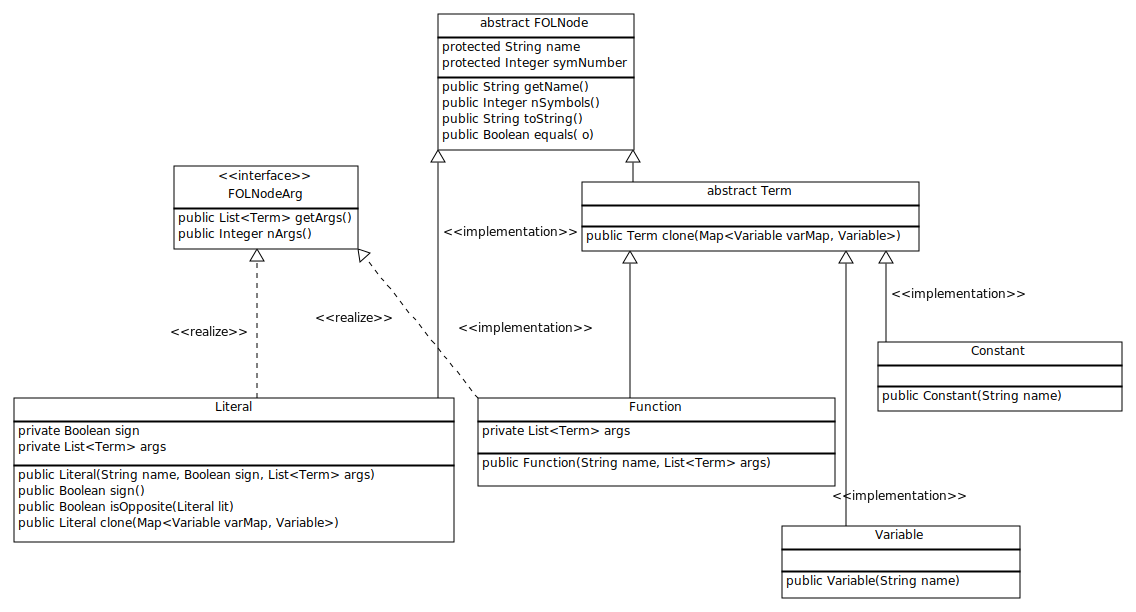
\includegraphics[width=1\columnwidth]{beanClassUML.png}
\caption{UML delle classi bean rilevanti}
\label{beanClassUML}
\end{figure}




Poiché si è deciso di mantenere il più possibile separate la fase di 
parsing e quella di implementazione dell'algoritmo di Nelson-Oppen, è 
stato necessario creare una classe “contenitore”, \texttt{CCObject} 
(\emph{src/bean}), in grado di mantenere sia i riferimenti a tutte le 
strutture dati create dal parser, sia alcune informazioni visualizzate 
in output (e.g. il numero di archi).\par
Per quanto riguarda le strutture dati, si è fatto un ingente uso di tavole 
hash tramite le classi \texttt{HashMap} ed \texttt{HashSet}; dove invece
è necessario mantenere l'ordine di inserimento, è stata utilizzata le 
struttura dati delle liste, tramite la classe \texttt{LinkedList}.\par
La scelta di utilizzare diffusamente tavole hash è avvalorata dal 
fatto che queste strutture, oltre a supportare le operazioni 
\texttt{insert}, \texttt{contains} e \texttt{remove} in tempo atteso 
costante, prevengono efficacemente la presenza di oggetti doppi nell'insieme.
In particolare il DAG è implementato tramite un \texttt{HashMap} le 
cui chiavi sono i campi \texttt{id} dei vari nodi.
Ciò permette di non dover mantenere, nelle altre strutture di supporto, 
il riferimento direttamente a tali nodi ma solamente le loro chiavi, sapendo 
che poi la ricerca all'interno del DAG avviene in maniera efficiente.

\subsection{Parser}
Dopo che la stringa è stata letta (inserita tramite riga di comando 
oppure prelevata da un file), il parser si preoccupa di farne un'analisi 
lessicale e sintattica per il riconoscimento di formule espresse 
nell'alfabeto $\Sigma_{E}\cup\Sigma_{cons}$, ovvero l'unione delle 
segnature della teoria dell'uguaglianza e delle liste (che ne è un 
estensione).\\
Il parser, che si può trovare nella cartella \emph{src/parser}, consiste 
in un file con estensione \texttt{.jj} costituito da un'unità di 
compilazione java e da una grammatica context-free di tipo \emph{LL(2)} 
le cui produzioni sono espresse in BNF (\emph{Backus–Naur Form}).
La grammatica è formata dalle seguenti categorie sintattiche: \\[1mm]
\begin{ttfamily}
\grammarindent Formula $::=$  Clause $($; Clause$?$ $)^*$ \\
\grammarindent Clause~ $::=$ Term = Term $|$ Term != Term $|$ atom(Term) $|$ -atom(Term) $|$ \\
\grammarindent[8] $($-$)?$ Pred(Term $($, Term$)^*$)\\
\grammarindent Term~~~ $::=$ cons(Term, Term) $|$ car(Term) $|$ cdr(Term) $|$ FunVar(Term $($, Term$)^*$) $|$ FunVar \\[1mm]
\end{ttfamily}
I token \texttt{Pred} e \texttt{FunVar} sono specificati dalle 
seguenti espressioni regolari:\\[1mm]
\begin{ttfamily}
\grammarindent Pred~~~ $::=$ $($["A"-"Z"]$)^+($["0"-"9"]$)^*$\\
\grammarindent FunVar~ $::=$ $($["A"-"Z"]$)^*($["a"-"z"]$)^+($["a"-"z","A"-"Z"]$)^*($["0"-"9"]$)^*$\\[1.5mm]
\end{ttfamily}
\noindent Considerazioni:
\begin{itemize}
\item il punto e virgola denota una congiunzione tra clausole;
\item sono stati utilizzati due caratteri diversi per la negazione 
solamente per ovviare ad un problema di compatibilità con la bash in caso 
l'input sia inserito da riga di comando; 
\item i simboli di predicato non interpretati sono espressi tramite 
lettere maiuscole mentre i simboli di funzione e di variabile con almento 
una lettera minuscola (opzionalmente possono anche essere seguiti da 
cifre);
\item ogni clausola identifica un unico predicato che è formato da uno o 
più termini; ogni termine può essere a sua volta formato da sottotermini 
oppure identificare un simbolo terminale, ovvero una variabile o una costante 
(nel frammento senza quantificatori si perde la distinzione fra queste due 
categorie sintattiche).
\end{itemize}
\par
Per quanto riguarda l'aspetto semantico, per ogni predicato e per ogni 
termine è stato inserito del codice Java che principalmente si occupa 
della costruzione del DAG, mantenuto tramite una tavola hash 
implementata utilizzando la classe \texttt{HashMap}. Il grafo è 
costruito mediante un approccio bottom-up.
\begin{itemize}
\item Ogni produzione di ciascun termine riceve uno o più oggetti di tipo 
\texttt{Node} (\emph{src/bean}) che rapprensentano i nodi del grafo dei 
suoi sottotermini; viene creato un nuovo nodo rappresentante quel termine 
ed si effettua il matching tra il suo campo \emph{argument} 
(\texttt{LinkedList}) ed il campo \emph{parent} (\texttt{HashSet}) 
dei suoi figli. Ciò avviene inserendo la chiave del nodo nei campi 
\emph{parent} dei figli e le chiavi dei figli nel campo \emph{argument} 
del padre.
\item Ogni produzione di ciascun predicato riceve anch'esso uno o più 
oggetti di tipo nodo ma si comporta in maniera diversa a seconda del 
tipo di predicato:
\begin{enumerate}[a)]
\item per quanto riguarda i predicati di uguaglianza, vengono 
semplicemente inserite le coppie di termini\footnote{Poichè si è reso 
necessario memorizzare i termini in coppia, è stato creata la classe 
\texttt{TermPair} (\emph{src/bean}) che tramite l'overriding dei 
metodi \texttt{hashCode} ed \texttt{equals} permette di mantenere coppie 
non ordinate nei vari \texttt{HashSet}.} in due insiemi a seconda che 
il predicato sia positivo o negativo;
\item per quanto riguarda il prediato \texttt{atom}, se è positivo 
il suo argomento viene inserito nell'insieme (\texttt{HashSet}) di tutti 
i termini che sono argomenti di \texttt{atom}, mentre se è negativo si effettua una 
trasformazione sintattica creando tre nuovi nodi: due variabili fresh 
ed un termine \texttt{cons} che ne diviene il padre; la coppia formata da 
questo nuovo nodo e dall'argomento del predicato viene poi aggiunta all'
insieme dei predicati di uguaglianza;
\item per quanto riguarda gli altri predicati non interpretati si 
effettua anche in questo caso una trasformazione sintattica in maniera 
da convertirli in fuzioni; li si inserisce poi nell'insieme dei 
predicati di uguagliaza o di disuguaglianza, a seconda che siano 
positivi o negativi, in coppia con un simbolo speciale che è stato 
scelto essere “\#”.
\end{enumerate}
\end{itemize}
\par
Per quanto riguarda le produzioni delle funzioni e dei predicati in cui 
il numero di argomenti non è noto a priori, si mantiene una corrispondenza 
(\texttt{HashMap}) tra i simboli letti ed il corrispettivo numero di 
argomenti. In questo modo, in caso si trovino due simboli uguali con un 
diverso numero di argomenti, viene sollevata un'eccezione.\\ 
Durante l'elaborazione di ogni nodo, vengono aggiornati anche tutti 
quei dati, come il numero di archi o di clausule di uguaglianza, che 
saranno poi forniti in output.
 
\subsection{Algoritmo di Nelson-Oppen}
Dopo che è stato effettuato il parsing dell'intera formula e creato il 
DAG, viene eseguito l'algoritmo di chiusura di congruenza di cui ne 
sono state implementate due versioni selezionabili dall'utente 
mediante l'eventuale uso dell'opzione \texttt{-h}.\par
La prima versione è la semplice trasposizione in codice Java 
dell'algoritmo presente al capitolo 9.3 del libro \emph{The Calculus 
of Computation} di A. R. Bradley e Z. Manna.\par
La seconda versione è una nuova reingegnerizzazione di tale algortimo 
tramite l'utilizzo di alcune euristiche atte soprattutto a permettere, 
non appena viene trovata una contraddizione tra due termini, l'immediata 
interruzione del flusso di esecuzione restituendo insoddisfacibile.\par
L'idea è quella di mantenere per ogni nodo un \emph{banned set} 
composto da tutti quei termini che non possono appartenere alla sua 
stessa classe di congruenza. Tale insieme viene popolato durante il 
parsing: ogniqualvolta si incontra un predicato di disuguaglianza 
$s_{i} \not= t_{i}$, viene aggiunto al \emph{banned set} del nodo che 
rappresenta $s_{i}$ il termine $t_{i}$ e viceversa. 
% Durante il parsing, per ogni termine che compone un predicato di disuguaglianza,
% si inserisce nel suo \emph{banned set} l'altro termine con cui forma tale predicato.
In questo modo ogni volta che due termini devono essere uniti in base 
agli assiomi di congruenza, si controlla se uno è nel \emph{banned 
set} dell'altro ed, in caso affermativo, si restituisce immediatamente 
insoddisfacibile. \par
Questa euristica può essere ulteriormente migliorata sulla base di questa 
considerazione: quando si effettua l'operazione di \texttt{merge} tra 
due nodi in realtà si stanno unendo le loro classi di congruenza e quindi 
è utile controllare non solo se i due termini formano un predicato di 
disuguaglianza, ma anche se nel \emph{banned set} di ciausun nodo vi è il 
riferimento ad uno dei nodi appartenenti alla stessa classe di congruenza 
dell'altro. Per implementare ciò, quando si effettua l'operazione di 
\texttt{union}, non si fa l'unione solamente tra i campi \texttt{ccpar}, 
ma anche tra i campi \texttt{banned}. In questo modo, ogniqualvolta 
viene eseguito il metodo \texttt{merge} tra due nodi, si controlla se è possibile 
unire le loro classi di congruenza: si seleziona il \emph{banned set} 
del rappresentante di uno dei due nodi e, per ogni termine presente in 
esso, si controlla se la sua classe di congruenza è la stessa classe dell'altro 
nodo con cui si vuole effettuare la \texttt{union} ritornando, in caso 
positivo, insoddisfacibile.
\begin{java}
// id1, id2 : nodes' id for which make union
for(String ban: node(find(id1)).getBanned())
		if(find(ban).equals(find(id2))) // CONFLICT
			return new TermPair(id1, id2);
\end{java}
Tale operazione è ripetuta simmetricamente anche per l'altro nodo e 
non peggiora la complessità dell'algoritmo in quanto è lineare sul numero
di nodi dei \emph{banned set}.\par 
Sulla base di questa euristica, che in pratica modifica i \emph{banned set} 
durante l'applicazione degli assiomi di congruenza, possiamo riformulare 
l'algoritmo di Nelson-Oppen.
\begin{enumerate}
\item Controllare che nessun argomento dei predicati \texttt{atom} sia un 
termine \texttt{cons}, in accordo con l'assioma \emph{(atom)} della teoria
delle liste. Se ne viene rilevata la presenza restituire UNSAT.
\item Aggiungere ai \emph{banned set} dei nodi che rappresentano gli 
argomenti del predicato \texttt{atom} tutti i termini \texttt{cons} (e 
viceversa) in modo da rispettare l'assioma precedente anche durante 
la propagazione degli effetti di nuove congruenze.
\item Per ogni nodo \texttt{cons} aggiungere al DAG due nuovi nodi 
\texttt{car} e \texttt{cdr} il cui archi puntano a quel nodo e 
poi effettuare la \texttt{merge} del \texttt{car} con il primo argomento 
del \texttt{cons} e del \texttt{cdr} con il secondo. In caso di conflitto
durante la \texttt{merge}, ritornare UNSAT.
\item Effettuare la \texttt{merge} di ogni coppia di termini presente 
nell'insieme dei predicati di uguaglianza. In caso di conflitto ritornare 
UNSAT. 
\item Ritornare SAT.
\end{enumerate}
Da notare che in realtà l'implementazione dell'algoritmo non ritorna 
insoddisfacibile bensì la coppia di termini tra i quali si è 
manifestato il conflitto. Inoltre la percentuale che si può osservare 
durante l'esecuzione, consiste nella percentuale del numero di clausole di 
uguaglianza fino a quell'istante computate.\par
Poichè l'algoritmo opera sui nodi del DAG come su una foresta di insiemi 
disgiunti, è possibile implementare altre due euristiche nei metodi 
\texttt{find} ed \texttt{union} in modo da abbassarne ulteriormente 
il tempo di esecuzione.
\begin{itemize}
\item {\bf Path Compression}: la compressione dei cammini, implementata 
nel metodo \texttt{find\_h}, consiste nell'appiattire la stuttura 
dell'albero che identifica ciascuna classe di congruenza facendo puntare
tutti i nodi direttamente al rappresentante; in questo modo le successive 
chiamate a tale funzione su quei nodi possono essere espletate in 
tempo costante. Per ottenere ciò si applica un metodo a doppio 
passaggio: durante il primo passaggio, il metodo risale ricorsivamente 
il cammino di ricerca per trovare la radice; durante il secondo passaggio, 
ridiscende il cammino di ricerca per aggiornare i nodi in modo che 
puntino direttamente al rappresenante.
\item {\bf Union by Rank}: l'unione per rango, implementata nel metodo 
\texttt{union\_h}, consiste nell'unire due classi di congruenza in 
modo che il nuovo rappresentante sia quello della classe più grande 
delle due. Il vantaggio è che i nodi della classe di congruenza che 
cambia rappresentante avranno una distanza maggiore dalla radice e 
quindi l'operazione di \texttt{find} sarà più onerosa. Per implementare 
ciò, ogni nodo è provvisto di un campo \texttt{rank} che è un limite 
superiore al numero di archi tra quel nodo e una foglia discendente.
Quando due classi di congruenza vengono unite, si trasforma il 
rappresentante di rango più alevato nel rappresentante di rango più basso, 
senza però modificare questo campo. Se invece i ranghi dei due 
rappresentanti sono uguali, se ne trasforma arbitrariamente uno nel 
padre dell'altro, incrementandone anche il rango.
\end{itemize}

%%%%%% Benchmark %%%%%%%%
\section{Benchmark}
In questa sezione viene riportata l'analisi dell prestazioni di tale 
algoritmo effettuata su un calcolatore con CPU \texttt{Intel Core 2 Duo 
P8600 2.4GHz}, sistema operativo \texttt{Ubuntu 10.10} e \texttt{JVM 
v1.6.0\_24}.\\
Le formule sono state create tramite un generatore automatico, 
\texttt{formulaGenerator}, che fa un ingente uso di una funzione random. 
Inoltre per automatizzare i test è stato implementato uno script 
(\texttt{generatorTest.sh}) che crea e salva i risultati in un file 
denominato \texttt{testResult.cvs}.\par
Di seguito sono presentate due tabelle con alcuni dei dati raccolti sulle 
prestazioni dell'algoritmo: la prima riguarda i test effettuati su formule 
composte da clausole miste, mentre la seconda su formule contenenti solo 
clausole di uguaglianza, \texttt{-atom} e predicati positivi che sono 
quindi forzatamente soddisfacibili.
\begin{table}[!htp]
\center
\begin{tabular}{llGcrr}
\toprule
Clausole & Nodi & Archi & Risultato & Time (ms) & Time eur (ms) \\
\midrule
64 & 415 & 1162 & UNSAT & 56 & 43 \\
384 & 1417 & 3809 & UNSAT & 14841 & 149 \\
512 & 1747 & 4926 & UNSAT & 8407 & 251 \\
768 & 2959 & 8359 & UNSAT & 40988 & 422 \\
1152 & 3581 & 10563 & UNSAT & 78023 & 328 \\
1408 & 6514 & 22319 & UNSAT & 997942 & 924 \\
\bottomrule
\end{tabular}
\caption{\footnotesize{Prestazioni dell'algoritmo su formule con 
clausole miste}}
\end{table}

\begin{table}[!htp]
\center
\begin{tabular}{llGcrr}
\toprule
Clausole & Nodi & Archi & Risultato & Time (ms) & Time eur (ms) \\
\midrule
64 & 427 & 1357 & SAT & 86 & 77 \\
512 & 2018 & 6111 & SAT & 21660 & 1598 \\
384 & 2381 & 8450 & SAT & 22064 & 2427 \\
1152 & 4108 & 11633 & SAT & 153478 & 5441 \\
768 & 4243 & 15041 & SAT & 124388 & 7663 \\
1408 & 8582 & 31080 & SAT & 1184730 & 34355 \\
\bottomrule
\end{tabular}
\caption{\footnotesize{Prestazioni dell'algoritmo su formule 
soddisfacibili}}
\end{table}
\subsection{Considerazioni}
Nelle tabelle sopra riportate si è deciso di ordinare le righe a 
seconda del numero di archi nel grafo visto che è su questa grandezza 
che viene calcolata la complessità. Dalla seconda tabella si può 
notare che non sempre ad un aumento del numero di clausole corrisponde 
un aumento del numero di archi: infatti il numero di nodi e di archi 
dipende principalmente dalla quantità di sottotermini presenti nella formula 
e questa grandezza varia in maniera casuale per ogni formula generata.\par
Dalle tabelle sopra riportate si può facilmente notare quanto 
l'algoritmo con euristiche sia più performante dell'altro quando le 
formule cominciano ad essere consistenti. Questo perché l'algoritmo originale 
non deve compiere attività di preprocessing (e.g. scorrere ed 
aggiornare i vari \emph{banned set}) per cui, quando il numero di archi 
è limitato, riescie ad essere più performante come nel caso del primo 
test della prima tabella. \par 
Quando invece la grandezza del DAG aumenta, tramite le euristiche si 
ottengono migliori performance: nei test di formule con clausole miste, 
poiché il risultato è sempre UNSAT, la differenza tra le prestazioni è 
dovuta principalmente all'euristica che fa uso dei \emph{banned set} 
per restituire insoddisfacibile non appena trova un conflitto. 
Nei test di formule soddisfacibili, invece, quest'euristica è 
inefficiente in quanto sicuramente non vi sono contraddizioni tra 
termini o predicati; la differenza di prestazioni rispetto all'algoritmo 
originale è, in questo caso, data dall'implementazione delle tecniche 
di unione per rango e compressione dei cammini dei metodi \texttt{union} 
e \texttt{find}.

\end{document}

